\documentclass[11pt]{article}
\usepackage{mathtools}
\usepackage{mdframed}
\usepackage{fullpage}
\usepackage{amsfonts}
\usepackage{tikz}
\usepackage{fancyhdr}
\usepackage{lastpage}
\usetikzlibrary{automata, positioning}


%edit this for each class
\newcommand\name{John Collin Vincent}
\newcommand\classname{Com S 331}
\newcommand\assignment{Homework 8}


\newcounter{excounter}
\setcounter{excounter}{1}
\newcommand\ques[2]{\vskip 1em  \noindent\textbf{\arabic{excounter}\addtocounter{excounter}{1}.} \emph{#1} \noindent#2}
\newenvironment{question}{\ques{}\begin{quote}}{\end{quote}}


\pagestyle{fancy}
\rfoot{\name, page \thepage/\pageref{LastPage}}
\cfoot{}
\rhead{}
\lhead{}
\renewcommand{\headrulewidth}{0pt}
\renewcommand{\footrulewidth}{0pt}
\DeclarePairedDelimiter\ceil{\lceil}{\rceil}
\DeclarePairedDelimiter\floor{\lfloor}{\rfloor}


\begin{document}


  {\bf \classname \hspace{1cm} \assignment\hfill \name}
  \vskip 2em


  \begin{question}
    \center
    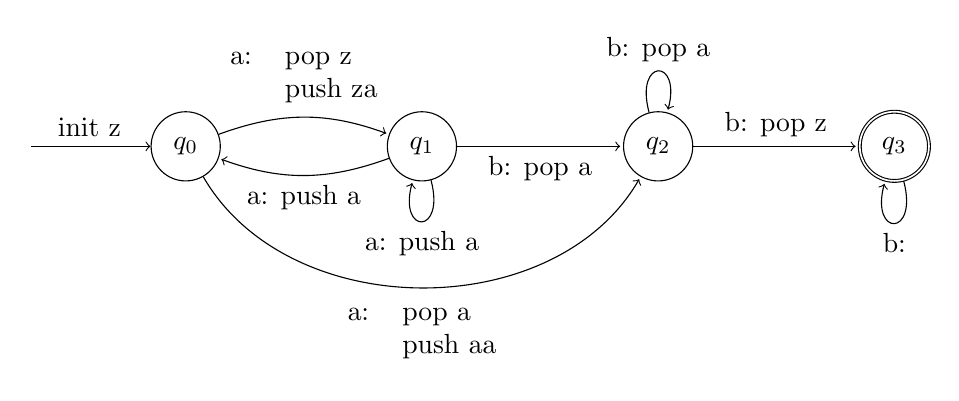
\begin{tikzpicture}[shorten >=1pt,node distance=3cm,on grid,auto]
      \node[state] (q_0) {$q_0$};
      \node[state] (q_1) [right=of q_0] {$q_1$};
      \node[state] (q_2) [right=of q_1] {$q_2$};
      \node[state, accepting] (q_3) [right=of q_2] {$q_3$};
      \draw[<-] (q_0) -- node[above] {init z} ++(-2cm, 0);
      \path[->]
      (q_0) edge [bend left=20] node [above] {\begin{tabular}{ll}a:&pop z\\&push za\end{tabular}} (q_1)
            edge [bend right=60] node [below] {\begin{tabular}{ll}a:&pop a\\&push aa\end{tabular}} (q_2);
      \path[->]
      (q_1) edge [loop below] node [below] {a: push a} ()
            edge [bend left=20] node [below] {a: push a} (q_0)
            edge node [below] {b: pop a} (q_2);
      \path[->]
      (q_2) edge [loop above] node [above] {b: pop a} ()
            edge  node [above] {b: pop z} (q_3);
      \path[->]
      (q_3) edge [loop below] node [below] {b: } ();
    \end{tikzpicture}
  \end{question}


\end{document}
